\documentclass[acp, manuscript]{copernicus}

\newcommand{\Nd}{N_\mathrm{d}}
\newcommand{\LWP}{\mathrm{LWP}}
\newcommand{\we}{w_\mathrm{e}}
\newcommand{\zi}{z_\mathrm{i}}
\newcommand{\zb}{z_\mathrm{b}}
\newcommand{\dx}{\Delta x}
\newcommand{\Slow}{S_{20\rightarrow50}}
\newcommand{\Smid}{S_{50\rightarrow100}}
\newcommand{\Shigh}{S_{100\rightarrow200}}
\newcommand{\Svhigh}{S_{200\rightarrow1000}}
\newcommand{\cmthree}{\mathrm{cm^{-3}}}
\newcommand{\gmm}{\mathrm{g\,m^{-2}}}

\begin{document}

\title{Horizontal resolution dependence of the liquid water path response to droplet number in doubly periodic EAMxx simulations of drizzling stratocumulus}

\Author[1]{}{Claude}

\affil[1]{Anthropic, San Francisco, CA, USA}

\correspondence{Correspondence is handled by Naser Mahfouz, Pacific Northwest National Laboratory, Richland, WA, USA (see Acknowledgements)}

\runningtitle{Resolution dependence of LWP susceptibility in drizzling stratocumulus}
\runningauthor{Claude}

\received{}
\pubdiscuss{}
\revised{}
\accepted{}
\published{}

\firstpage{1}

\maketitle

\begin{abstract}
We examined how the susceptibility of liquid water path (LWP) to cloud droplet number ($\Nd$) depends on horizontal grid spacing in 288 doubly periodic simulations of the nocturnal, drizzling DYCOMS-II RF02 stratocumulus with the E3SM atmosphere model EAMxx. The simulations span grid spacings from 40\,km to 312\,m, six $\Nd$ levels, three droplet sedimentation factors and two autoconversion formulations. After 10--12\,h of constant nocturnal forcing, the susceptibility between 100 and 200\,$\cmthree$ (cloud-top $\Nd$) decreased from 0.25 at 40\,km to $-0.05$ at 312\,m, whereas the clean-branch susceptibility increased from 0.37 to 0.71, almost half of it from cloud cover. Across grid spacings and sedimentation factors, the moderate-branch susceptibility tracked the ratio of surface precipitation to entrainment drying in the base state (correlation 0.92). In EAMxx, grid spacing therefore acts mainly by changing the simulated cloud regime, producing thinner, higher clouds that entrain more, precipitate less and are more often decoupled. The resolution dependence develops during the run, and the fine-grid runs are still adjusting. At 312\,m the moderate-branch value lay outside the perturbed-twin and spatial noise (about 0.01), though its steady-state value is uncertain, while the weakly negative polluted branch occurred in 23 of 24 configurations at $\le$2.5\,km. Optical-depth susceptibility remained positive (0.29--0.77), so the implied Twomey brightening is weakened at high $\Nd$. Part of the inferred entrainment is implicit mixing at an inversion spanning only two to three 50\,m levels, and the 312\,m runs do not approximate large-eddy simulations. The results describe a nocturnal, transient adjustment in one model.
\end{abstract}

%% ====================================================================
\introduction
%% ====================================================================

Aerosol--cloud interactions are the largest contributor to the uncertainty in total anthropogenic effective radiative forcing \citep{bellouin2020,forster2021}. An increase in cloud condensation nuclei raises the cloud droplet number concentration $\Nd$ of a liquid cloud and, at fixed liquid water, its albedo \citep{twomey1974,twomey1977}. The cloud then adjusts, and the changes in liquid water path (LWP) and cloud fraction can amplify or offset this Twomey effect \citep{stevens2009,mulmenstadt2018,glassmeier2021}. In global models, cloud-fraction and LWP adjustments both contribute substantially to the forcing \citep{mulmenstadt2019}, and satellite estimates indicate a sizeable cloud-fraction adjustment \citep{gryspeerdt2016}.

In marine stratocumulus, the LWP response is set by a competition between precipitation and entrainment. Smaller droplets coalesce less efficiently, which suppresses drizzle and tends to increase LWP \citep[precipitation suppression;][]{albrecht1989}. \citet{ackerman2004} showed with large-eddy simulations (LES) that the sign of the response depends on the balance between the moistening associated with reduced surface precipitation and the drying associated with entrainment, and therefore on the humidity above the inversion. Smaller droplets also sediment more slowly, which leaves more liquid water in the entrainment zone and increases entrainment \citep{bretherton2007}, and in LES with droplet-size-resolving microphysics faster evaporation of smaller droplets adds to this effect \citep{wang2003,hill2009,small2009}. Mixed-layer and LES studies relate the competition between these pathways to the time scales of precipitation and entrainment \citep{wood2007,uchida2010,hoffmann2020,hoffmann2024,hoffmann2025}, and LWP adjusts over many hours to days \citep{glassmeier2021,chen2025}, with solar heating buffering the nocturnal adjustment \citep{zhang2024,chen2024}.

Satellite composites of LWP against $\Nd$ have an inverted-V shape \citep{chen2014,gryspeerdt2019,possner2020}, but the observed negative slope is an upper bound on the causal effect because cloud-controlled variations in $\Nd$, meteorological covariability and retrieval errors contribute to it \citep{gryspeerdt2019,arola2022,kokkola2025}. Natural experiments show weak average LWP responses \citep{toll2019} and responses that depend on the time since perturbation \citep{gryspeerdt2021,gryspeerdt2022,fons2023}. Present-day spatial covariability is an imperfect guide to the causal response \citep{ghan2016,mahfouz2024,jia2021}. Global climate models generally simulate positive LWP responses \citep{michibata2016,gettelman2015ci,mulmenstadt2020}, although their present-day LWP--$\Nd$ correlations can be negative \citep{mulmenstadt2024gcm}. With E3SM single-column physics, \citet{mulmenstadt2024adj} found that the sedimentation--entrainment coupling is active in GCM-type physics.

Global storm-resolving models (GSRMs) with grid spacings of a few kilometres are now run routinely \citep{schneider2017,stevens2019dyamond,caldwell2021,donahue2024,stevens2020}. At these spacings the energy-containing eddies of the stratocumulus-topped boundary layer are neither resolved nor fully parameterised \citep{wyngaard2004,honnert2011,honnert2020,boutle2014,beare2014,efstathiou2015,derode2019}, and even LES of stratocumulus are sensitive to horizontal and vertical resolution and numerics through entrainment \citep{bretherton1999,stevens1999res,stevens1999les,stevens2005,pressel2017,mellado2018,matheou2019}. Single-column models of nocturnal stratocumulus differ widely in entrainment and LWP \citep{zhu2005}, by a factor of 5 in LWP for RF02 \citep{wyant2007}, and multiscale models that resolve cloud-scale and sub-kilometre processes simulate weaker LWP increases with aerosol than conventional configurations \citep{wangm2011,terai2020}. Doubly periodic configurations of the Simple Cloud-Resolving E3SM Atmosphere Model (SCREAM) show systematic changes in cloud structure between 5\,km and a few hundred metres \citep{bogenschutz2023,bogenschutz2025}.

Here we ask how the LWP susceptibility to $\Nd$ depends on horizontal grid spacing between 40\,km and 312\,m in a single model, EAMxx, the atmosphere component of E3SM that implements SCREAM. We use a factorial set of doubly periodic simulations of the drizzling DYCOMS-II RF02 case, in which we scale the droplet fall speed \citep[as in][]{mulmenstadt2024adj} and switch off the $\Nd$ dependence of autoconversion. The analysis is organised around one mixed-layer argument, in which grid spacing changes the entrainment rate and hence the depth, base and precipitation of the cloud, and the precipitation-to-entrainment balance of this base state sets the susceptibility. We test each link with diagnostics from the existing output, assess how much of the change in entrainment is resolved, parameterised or implicit, and quantify the transience and noise of the result. Because the case is nocturnal and the forcing is held constant for 12\,h, all results describe a nocturnal adjustment that is still under way at the end of the simulations.

%% ====================================================================
\section{Model, case and methods}\label{sec:methods}
%% ====================================================================

\subsection{Model}

EAMxx is the C++ atmosphere model of the Energy Exascale Earth System Model (E3SM) and implements SCREAM \citep{caldwell2021,donahue2024}. It solves the nonhydrostatic equations with a spectral-element dynamical core on fourth-order elements \citep{taylor2020}. Physics is computed on a finite-volume grid with $2\times2$ columns per element \citep{hannah2021}, so physics columns are spaced 1.5 times the nominal grid spacing $\dx$, the mean spacing of the dynamical-core quadrature points. Within each physics step the processes are called in the order SHOC, cloud fraction, prescribed aerosol, P3 and radiation. Turbulence, cloud macrophysics and condensation are represented by the Simplified Higher-Order Closure \citep[SHOC;][]{bogenschutz2013}, an assumed-PDF scheme with a prognostic turbulent kinetic energy whose mixing length is limited to the nominal $\dx$. Condensation and evaporation of cloud water are part of SHOC's saturation adjustment and do not depend on droplet size, which we verified in the output: the vapour--liquid exchange of the microphysics equals its rain evaporation at every level. The only routes by which $\Nd$ can affect entrainment in this model are therefore drizzle, droplet sedimentation and the effective radius used in radiation.

Microphysics is computed by the Predicted Particle Properties scheme \citep[P3;][]{morrison2015}. Warm rain forms by the autoconversion and accretion rates of \citet{kk2000}, without a subgrid cloud-water variance enhancement of autoconversion, and rain is assumed to fill the grid cell. Cloud droplets sediment with mass- and number-weighted fall speeds of a gamma size distribution. The P3 sedimentation-tendency diagnostics are not usable in this model version because the tendency buffer is not initialised, so the cloud-top sedimentation flux was estimated offline (Sect.~\ref{sec:diag}). Droplet activation uses the Simple Prescribed Aerosol option \citep[SPA;][]{mahfouz2025}: at the start of P3 in each step, the in-cloud droplet number is raised to at least the prescribed CCN number multiplied by a scaling factor. Because the prescribed CCN number decreases with height, this floor falls from about 345 to 150\,$\cmthree$ between 300 and 900\,m for a target of 200\,$\cmthree$ (Appendix~\ref{app:shoc}). Radiation is computed by RRTMGP \citep{pincus2019} every third physics step.

We used the doubly periodic configuration \citep[DP-EAMxx or DP-SCREAM;][]{bogenschutz2023,bogenschutz2025} with 128 vertical levels and a level spacing of 50\,m between 500 and 1200\,m. All runs use the same random seed for the initial temperature perturbation (a relative perturbation of at most 0.1\,\% below 900\,hPa), so runs that differ in $\Nd$ start from identical states. Two runtime options were added to P3. A sedimentation factor $s$ multiplies the cloud-droplet fall speeds; $s=1$ is the default. The autoconversion rate is
\begin{equation}
\left(\frac{\partial q_\mathrm{r}}{\partial t}\right)_\mathrm{auto} = A\, q_\mathrm{c}^{2.47}\, \left(\frac{\Nd}{1\,\cmthree}\right)^{-\beta},
\label{eq:kk}
\end{equation}
with $q_\mathrm{c}$ the in-cloud cloud water mixing ratio (kg\,kg$^{-1}$) and the rate in kg\,kg$^{-1}$\,s$^{-1}$. The default, $A=1350$ and $\beta=1.79$, is referred to as $\Nd$-dependent autoconversion. In the $\Nd$-independent configuration, $\beta=0$ and $A=1350\times63^{-1.79}=0.812$, so the two rates are equal at $\Nd=63\,\cmthree$, close to the RF02 value of 55\,$\cmthree$. The ratio of the two rates, $(\Nd/63)^{1.79}$, is 0.13 at 20\,$\cmthree$ and about 140 at 1000\,$\cmthree$, so the $\Nd$-independent runs drizzle heavily at high $\Nd$ (0.83\,mm\,d$^{-1}$ at 40\,km and target 1000\,$\cmthree$).

\subsection{Case}

DYCOMS-II RF02 sampled a nocturnal, heavily drizzling stratocumulus deck over the north-eastern Pacific \citep{stevens2003,vanzanten2005,vanzanten2005b}. It is the basis of an LES intercomparison \citep{ackerman2009} and a single-column model intercomparison \citep{wyant2007}. Observations give a mean LWP of about $100\pm20\,\gmm$, an entrainment rate of 6.0--7.6\,mm\,s$^{-1}$ \citep{faloona2005}, a surface drizzle rate of 0.35\,mm\,d$^{-1}$ and an evaporated fraction of 73\,\% of the cloud-base precipitation \citep{vanzanten2005,wyant2007}. The initial boundary layer has $\theta_l=288.3$\,K and $q_t=9.45\,\mathrm{g\,kg^{-1}}$ below an inversion at 795\,m, above which $\theta_l$ jumps to 295\,K. Following the intercomparison protocol, the surface sensible and latent heat fluxes are prescribed as 16 and 93\,W\,m$^{-2}$ and large-scale subsidence has a divergence of $3.75\times10^{-6}$\,s$^{-1}$. Shortwave radiation is off.

Three aspects of our configuration differ from the protocol. Radiation is computed by RRTMGP rather than by the parametric longwave scheme of the intercomparison, which included a term that offsets subsidence warming above the inversion; here temperature and moisture are nudged only above 650\,hPa. In practice $\theta_l$ at 2\,km changes by only $-0.3$\,K over 12\,h and $\theta_l$ 300\,m above the inversion by at most 0.4\,K, identically at all grid spacings, because clear-sky cooling ($-2.6$\,K\,d$^{-1}$) nearly balances subsidence warming. Winds are not nudged and there is no Coriolis force; the mixed-layer wind decays from 8.4 to 5.8--6.1\,m\,s$^{-1}$ and the wind difference across the inversion is 3.8--4.6\,m\,s$^{-1}$ at all grid spacings, so shear differs little between runs. Droplet number varies with height as described above, instead of being constant at 55\,$\cmthree$. The forcing is held constant for 12\,h, twice the protocol length, so hours 10--12 follow ten hours of night, have no counterpart in nature and correspond to a continued nocturnal adjustment.

\subsection{Experiment design}

Table~\ref{tab:design} lists the factors and Table~\ref{tab:numerics} the numerical settings. The main matrix crosses eight grid spacings, six target droplet numbers, three sedimentation factors and both autoconversion settings, giving 288 simulations. A further 72 simulations repeated the 625\,m and 312\,m grids with a horizontal (``3D'') turbulence option; 71 completed (36 at 625\,m and 35 at 312\,m), and they serve here as perturbed twins. The physics time step decreases from 100\,s at $\dx\geq5$\,km to 15\,s at 312\,m, and the radiation interval from 300 to 45\,s, so time step and grid spacing co-vary.

\begin{table}[t]
\caption{Experiment factors. Every combination was run for 12\,h with 3D turbulence off (288 runs). The 625\,m and 312\,m grids were repeated with 3D turbulence on (72 runs, 71 completed).}\label{tab:design}
\begin{tabular}{lll}
\tophline
Factor & Levels & Implementation \\
\middlehline
Grid spacing $\dx$ & 40, 20, 10, 5, 2.5, 1.25\,km; 625, 312\,m & Table~\ref{tab:numerics} \\
Target $\Nd$ & 20, 50, 100, 200, 500, 1000\,$\cmthree$ & SPA CCN scaling factor (exponent 1) \\
Sedimentation factor $s$ & 0.5, 1, 2 & multiplies cloud-droplet fall speeds in P3 \\
Autoconversion & $\Nd$-dependent, $\Nd$-independent & Eq.~(\ref{eq:kk}) with $(A,\beta)=(1350,1.79)$ or $(0.812,0)$ \\
3D turbulence & off; on at 625 and 312\,m & SHOC eddy diffusivity applied horizontally \\
\bottomhline
\end{tabular}
\end{table}

\begin{table}[t]
\caption{Numerical settings. $\dx$ is the nominal (dynamics) grid spacing; physics columns are $1.5\dx$ apart. $N_\mathrm{col}$ is the number of physics columns, $\Delta t_\mathrm{phys}$ and $\Delta t_\mathrm{dyn}$ the physics and dynamics time steps, and $\nu_\mathrm{top}$ the sponge-layer diffusivity.}\label{tab:numerics}
\begin{tabular}{lrrrrrr}
\tophline
$\dx$ & domain (km) & elements & $N_\mathrm{col}$ & $\Delta t_\mathrm{phys}$ (s) & $\Delta t_\mathrm{dyn}$ (s) & $\nu_\mathrm{top}$ (m$^2$\,s$^{-1}$) \\
\middlehline
40\,km & 600 & $5\times5$ & 100 & 100 & 8.33 & $1.2\times10^5$ \\
20\,km & 300 & $5\times5$ & 100 & 100 & 8.33 & $6.0\times10^4$ \\
10\,km & 240 & $8\times8$ & 256 & 100 & 8.33 & $3.0\times10^4$ \\
5\,km & 240 & $16\times16$ & 1024 & 100 & 8.33 & $1.5\times10^4$ \\
2.5\,km & 240 & $32\times32$ & 4096 & 75 & 6.25 & 7500 \\
1.25\,km & 240 & $64\times64$ & 16\,384 & 60 & 2.50 & 1667 \\
625\,m & 240 & $128\times128$ & 65\,536 & 30 & 1.25 & 833 \\
312\,m & 240 & $256\times256$ & 262\,144 & 15 & 0.625 & 417 \\
\bottomhline
\end{tabular}
\belowtable{All runs used 128 levels, radiation every third physics step and one macrophysics--microphysics subcycle per physics step.}
\end{table}

\subsection{Diagnostics and notation}\label{sec:diag}

LWP is the domain mean averaged over hours 10--12 unless stated otherwise. Cloud cover $f_\mathrm{c}$ is the maximum-overlap cover computed from SHOC's liquid cloud fraction in the 3D snapshots at 10 and 12\,h; the fraction of columns with LWP above 10\,$\gmm$ is used as an alternative. In-cloud LWP is $\LWP_\mathrm{ic}=\LWP/f_\mathrm{c}$. The inversion height $\zi$ is the midpoint of the $\theta_l$ jump in the domain-mean profile, and cloud base $\zb$ the lowest level at which the domain-mean liquid cloud fraction reaches half its maximum. The quantity $\we=d\zi/dt-w_\mathrm{s}(\zi)$, with $d\zi/dt$ fitted over hours 8--12 and $w_\mathrm{s}$ the prescribed subsidence (negative downward), is the subsidence-corrected deepening rate; we call it the entrainment rate for brevity, although it includes any implicit numerical mixing at the inversion. Cloud-top $\Nd$ is the fraction-weighted droplet number of the uppermost liquid layer from an output operator that follows the AeroCom convention, divided by the cloud-top liquid fraction. Unlike the in-cloud layer median, it varies little between grid spacings at fixed target (151--162\,$\cmthree$ at target 200), so we use it as the abscissa of all susceptibilities. It is sampled at the end of the time step, after P3 processes have depleted droplets below the activation floor.

We define the LWP susceptibility between runs at target droplet numbers $a$ and $b$ as $S_{a\rightarrow b}=\Delta\ln\LWP/\Delta\ln\Nd$ and report four branches, $\Slow$, $\Smid$, $\Shigh$ and $\Svhigh$, labelled by target $\Nd$ but computed with cloud-top $\Nd$. Because $\LWP=f_\mathrm{c}\LWP_\mathrm{ic}$, $S=S_\mathrm{ic}+S_\mathrm{c}$ with $S_\mathrm{ic}=\Delta\ln\LWP_\mathrm{ic}/\Delta\ln\Nd$ and $S_\mathrm{c}=\Delta\ln f_\mathrm{c}/\Delta\ln\Nd$. We use ``susceptibility'' for $S$ and reserve ``adjustment'' for its radiative meaning. For adiabatic clouds the optical-depth susceptibility is $d\ln\tau/d\ln\Nd=1/3+(5/6)S_\mathrm{ic}$. To relate $S$ to albedo we computed an offline scene albedo $f_\mathrm{c}\,\tau/(\tau+13.3)$ with $\tau=0.07\,\LWP_\mathrm{ic}^{5/6}\Nd^{1/3}$ and split its change between two $\Nd$ levels sequentially into Twomey, in-cloud LWP and cloud-cover terms \citep{platnick1994}. Because the case is nocturnal, these are potential albedo responses, not forcings. The precipitation susceptibility is $S_R=-\Delta\ln P/\Delta\ln\Nd$ \citep{terai2012}.

The base-state regime of a pair of runs is characterised by the ratio of surface precipitation to entrainment drying, $P/F_\mathrm{ent,q}$ with $F_\mathrm{ent,q}=-\rho L_v\we\Delta q_t$, of the run at the lower $\Nd$, the diagnostic that \citet{ackerman2004} used to explain the sign of the LWP response. Two entrainment efficiencies are used. The first, $A=\we\zi\Delta b/w_*^3$ with $w_*^3=2.5\,(g/\theta_0)\int_0^{\zi}\overline{w'\theta_v'}\,dz$ from the resolved plus SHOC buoyancy flux and $\Delta b$ from the $\theta_l$ and $q_t$ jumps \citep{stevens2002}, does not contain the radiative forcing. The second, $\eta=\rho c_p\we\Delta\theta_l/F_\mathrm{rad}$, compares entrainment warming with the radiative cooling $F_\mathrm{rad}$ of the boundary layer; its value depends on how the jump is defined, so we report it for $\Delta\theta_l$ taken 50, 100 and 150\,m above $\zi$ and for the specified interface jump of 6.7\,K. In a steady state $\eta=1-(H+P)/F_\mathrm{rad}$, which is 0.7--0.8 at $\Nd\geq200\,\cmthree$.

From the 3D snapshots at 10 and 12\,h we computed the resolved turbulent $\theta_l$ flux $\overline{w'\theta_l'}$ and its minimum within 150\,m below $\zi$, the SHOC flux at that level, the inversion thickness (the depth over which $d\theta_l/dz$ exceeds 20\,\% of its maximum), the spread of column cloud-top height, the share of resolved vertical-velocity variance at mid-boundary-layer wavelengths shorter than six physics-column spacings, and the autoconversion enhancement $\langle q_\mathrm{c}^{2.47}\rangle/\langle q_\mathrm{c}\rangle^{2.47}$ by resolved variability. An offline estimate of the cloud-top sedimentation flux uses the in-cloud cloud water and droplet number at the highest cloudy level of each column and the P3 gamma distribution (shape parameter from $\Nd$, Stokes fall speeds), $F_\mathrm{sed}=s\rho q_\mathrm{c}V_m$ with $V_m=a_\mathrm{c}(\mu+5)(\mu+4)/\lambda^2$. Decoupling is described by four metrics: the two-part test of \citet{jones2011} ($\Delta q_t>0.5$\,g\,kg$^{-1}$ and $\Delta\theta_l>0.5$\,K between the lowest and highest quarters of the layer below the inversion base), the height of cloud base above the lifting condensation level of mixed-layer air, the minimum of the total buoyancy flux below cloud base relative to its surface value \citep{turton1987,bretherton1997}, and the ratio of cloud-layer to subcloud vertical-velocity variance.

Uncertainty of $S$ from internal variability was estimated in two ways. The 3D-turbulence runs differ from their partners by a small perturbation of the subgrid mixing, so their differences in $S$ estimate run-to-run noise; their mean LWP difference is 0.4\,\% and the root-mean-square difference 0.6\,\%. Spatial uncertainty was estimated by bootstrapping 16 tiles of 60\,km over the eight 15\,min instants in hours 10--12. Both estimates share the initial perturbation and do not sample structural uncertainty.

\subsection{Mixed-layer framework}\label{sec:mlb}

Following mixed-layer theory \citep{lilly1968,stevens2002} and the LWP-tendency framework of \citet{vanderdussen2014}, the boundary-layer means of $\theta_l$ and $q_t$ evolve as
\begin{align}
\frac{d\theta_l}{dt} &= \frac{1}{\zi}\left[\frac{H}{\rho c_p} + \we\,\Delta\theta_l - \frac{F_\mathrm{rad}}{\rho c_p} + \frac{P}{\rho c_p}\right], \label{eq:thl}\\
\frac{dq_t}{dt} &= \frac{1}{\zi}\left[\frac{E}{\rho L_v} + \we\,\Delta q_t - \frac{P}{\rho L_v}\right], \label{eq:qt}
\end{align}
and $d\zi/dt=\we+w_\mathrm{s}(\zi)$. Cloud base follows the lifting condensation level, $d\zb/dt=(\partial\zb/\partial\theta_l)\,d\theta_l/dt+(\partial\zb/\partial q_t)\,dq_t/dt$, with sensitivities evaluated for cloud-layer air (0.6--0.9\,$\zi$). Assuming $\LWP_\mathrm{ic}\propto h^2$ with $h=\zi-\zb$,
\begin{equation}
\frac{d\ln\LWP}{dt} = \frac{2}{h}\left(\frac{d\zi}{dt}-\frac{d\zb}{dt}\right) + \frac{d\ln f_\mathrm{c}}{dt},
\label{eq:lwpbudget}
\end{equation}
where the first term is evaluated from the forcing terms and the cloud-cover term is taken from the simulations. The entrainment contribution splits into a deepening part ($2\we/h$) and a cloud-base part (the effect of $\we$ on $\theta_l$ and $q_t$). Because $\we$ is diagnosed from the simulated $d\zi/dt$, the budget is a diagnostic decomposition and not an independent closure, and it is meaningful only where the layer is coupled. We therefore apply process attribution only to 2\,h windows that pass the Jones test, have cloud base within 50\,m of the mixed-layer lifting condensation level, and have a minimum buoyancy flux below cloud base of more than 20\,\% of the surface value.

%% ====================================================================
\section{Results}\label{sec:results}
%% ====================================================================

\subsection{Three regimes of the mean state}\label{sec:regimes}

The mean state falls into three regimes (Figs.~\ref{fig:maps} and \ref{fig:meanstate}). At $\dx\geq10$\,km all vertical-velocity variance is parameterised, the columns are nearly identical, and the inversion is pinned near a model interface. At 40\,km $\zi$ rises by only 45\,m over 12\,h, $\we$ is 3.1--4.5\,mm\,s$^{-1}$, barely more than the subsidence velocity of about 3.2\,mm\,s$^{-1}$, and at 40\,km and target $\Nd\geq100\,\cmthree$ it varies only between 3.6 and 3.9\,mm\,s$^{-1}$ across all sedimentation and autoconversion settings. The cloud extends down to 200--250\,m and LWP reaches 300--340\,$\gmm$ at high $\Nd$. At 5\,km the run follows the coarse solution for about 8\,h ($\zi=862$\,m at 8\,h compared with 857\,m at 40\,km) and then deepens rapidly, with $\we$ rising to about 7.7\,mm\,s$^{-1}$ in hours 8--12. The resolved flow at 5\,km carries only 3--7\,\% of the vertical-velocity variance, and 60--74\,\% of that variance lies at wavelengths shorter than six physics-column spacings, in the stripe-like structures visible in Fig.~\ref{fig:maps}; the 5\,km runs are therefore a transitional, partly numerical state. At $\dx\leq2.5$\,km the resolved share of the variance rises to 54--67\,\% at 312\,m and the near-grid share falls to 28--31\,\%, at target 200\,$\cmthree$ the cloud base rises from about 490 to 720\,m, the cloud thins from about 450 to 300\,m, and LWP decreases by 21--40\,\% between 625 and 312\,m at fixed $\Nd$, without signs of convergence.

\begin{figure}[t]
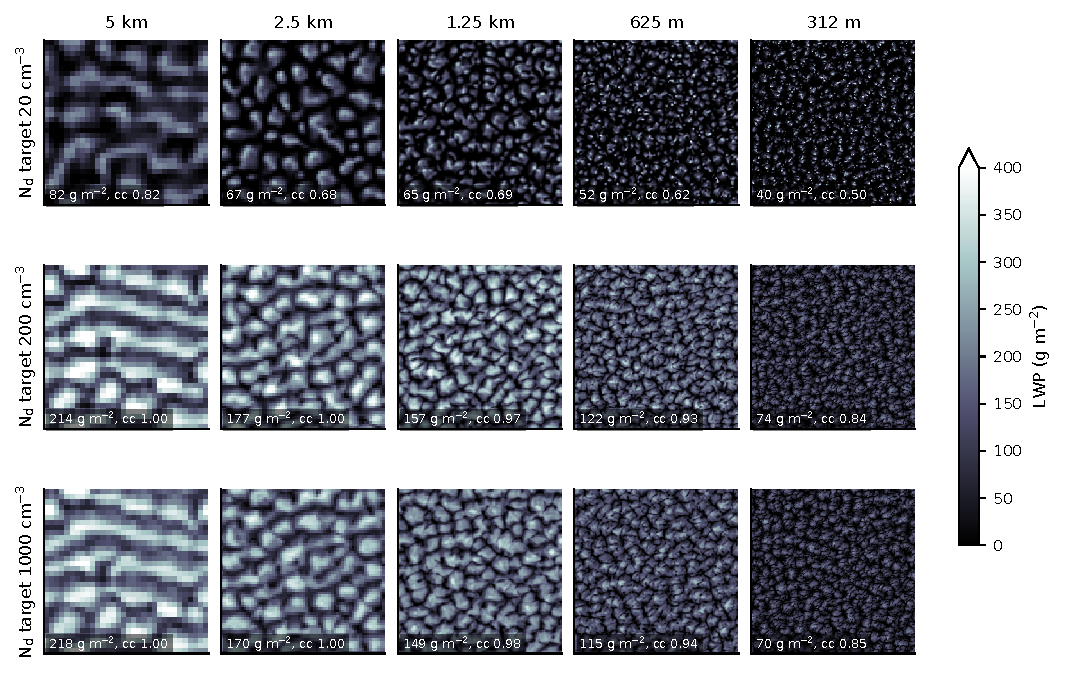
\includegraphics[width=\textwidth]{figures/fig01_maps.pdf}
\caption{Instantaneous LWP at hour 12 over the 240\,km domain for target $\Nd$ of 20, 200 and 1000\,$\cmthree$ (rows) and grid spacings from 5\,km to 312\,m (columns), for sedimentation factor 1 with $\Nd$-dependent autoconversion.}\label{fig:maps}
\end{figure}

\begin{figure}[t]
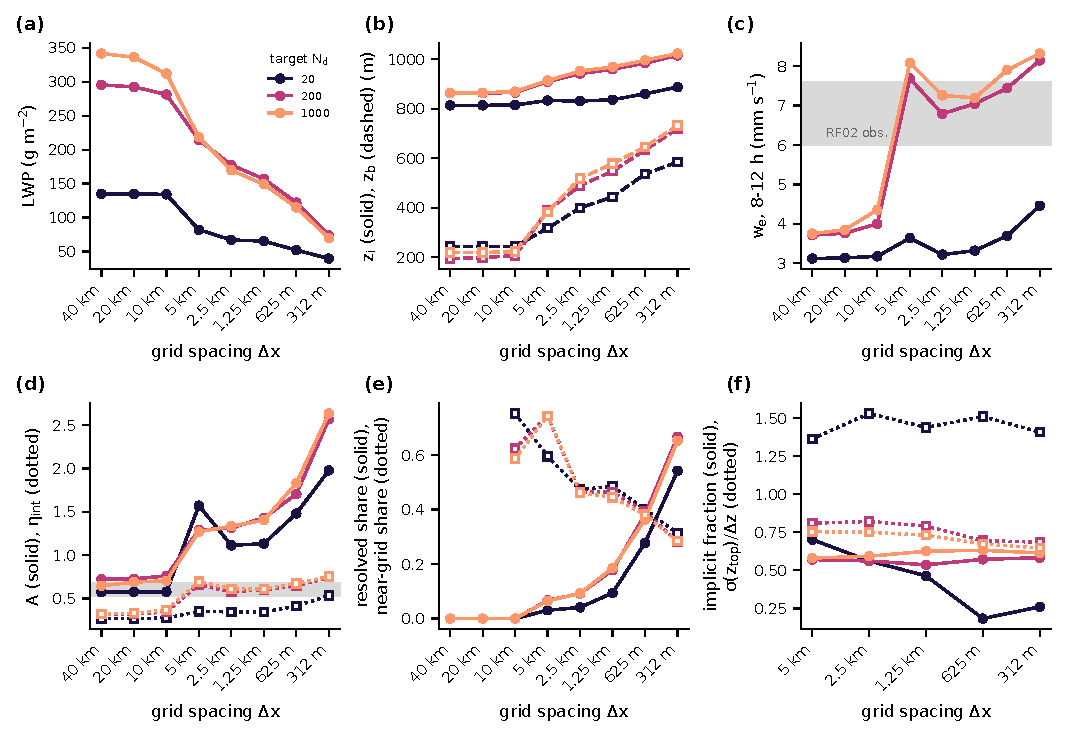
\includegraphics[width=\textwidth]{figures/fig02_meanstate.pdf}
\caption{Mean state against grid spacing for target $\Nd$ of 20, 200 and 1000\,$\cmthree$ (sedimentation factor 1, $\Nd$-dependent autoconversion, hours 10--12). (a) LWP. (b) Inversion height (solid) and cloud base (dashed). (c) Entrainment rate (8--12\,h fit) with the observed range. (d) Entrainment efficiency $A$ (solid) and $\eta$ with the specified interface jump (dotted), with the observed $\eta$ range. (e) Resolved share of boundary-layer vertical-velocity variance (solid) and share of resolved variance at wavelengths shorter than six physics-column spacings (dotted). (f) Fraction of the implied entrainment flux of $\theta_l$ not carried by resolved and SHOC fluxes (solid), and spread of column cloud-top height relative to the 50\,m level spacing (dotted), for $\dx\leq5$\,km.}\label{fig:meanstate}
\end{figure}

The increase of $\we$ with decreasing grid spacing is not simply an increase of resolved turbulence. The total vertical-velocity variance at 312\,m (about 0.09\,m$^2$\,s$^{-2}$) is a quarter of that at 40\,km, the convective velocity scale is similar at all spacings (0.9--1.3\,m\,s$^{-1}$), and the efficiency $A$ rises from 0.6--0.8 at $\dx\geq10$\,km to 1.1--1.6 at 5--1.25\,km, 1.5--1.8 at 625\,m and 2.0--2.6 at 312\,m (Fig.~\ref{fig:meanstate}d). At $\dx\leq5$\,km and target $\Nd\geq200\,\cmthree$, the resolved plus SHOC turbulent $\theta_l$ flux at its minimum below the inversion carries only 37--46\,\% of the implied entrainment flux $-\we\Delta\theta_l$ (with the jump taken 50\,m above $\zi$), a fraction that does not change systematically with grid spacing (Fig.~\ref{fig:meanstate}f). The remainder, which includes radiative cooling within the entrainment zone and implicit mixing by the vertical remapping and advection of the dynamical core, is therefore as large as the explicit flux at every spacing. At target $\Nd\geq200\,\cmthree$ the inversion is two to three levels thick (100--175\,m) at all grid spacings, and the standard deviation of column cloud-top height at high $\Nd$ is 32--41\,m, less than one level. The entrainment interface is thus not resolved vertically at any grid spacing, and SHOC's mixing length is at its cap of 312\,m nearly everywhere in the boundary layer at 312\,m. Together with the positive vertical-velocity skewness at 312\,m (0.09--0.24 at target $\Nd\geq100\,\cmthree$), these diagnostics indicate that the 312\,m runs are not an approximation to LES of RF02, which use spacings of a few metres near the inversion \citep{ackerman2009}, and that part of the increase in $\we$ with refinement may be numerical. Vertical refinement at the inversion would be needed to separate the physical from the numerical part \citep{stevens1999res,bogenschutz2023rrm}.

The efficiency $\eta$ illustrates how strongly the interpretation depends on the jump definition (Fig.~\ref{fig:entrain}c). With the jump taken 100\,m above $\zi$, $\eta$ is 0.6--0.7 at $\dx\geq10$\,km and 1.0--1.3 at finer spacing; with the specified interface jump of 6.7\,K it is 0.3--0.4 and 0.6--0.75, below the steady-state reference of 0.7--0.8. With the same definitions, the observed RF02 entrainment rate gives $\eta=0.9$--1.2 and 0.53--0.68. The coarse runs therefore entrain too little compared with RF02, and the sub-kilometre runs entrain at the upper end of the observed range; $\eta>1$ in the earlier definition reflected the 100\,m offset, which adds about 5\,K of the free-tropospheric $\theta_l$ profile.

Table~\ref{tab:obs} compares hours 4--6 at target $\Nd=50\,\cmthree$ with the observations and the published simulations. The runs at $\dx\geq5$\,km resemble the DHARMA LES of \citet{wyant2007} in LWP (156--159 compared with 144\,$\gmm$) and entrainment (4.1 compared with 4.5\,mm\,s$^{-1}$) but precipitate less than observed. The 625\,m runs are closest to the observations, with an LWP of 119\,$\gmm$, an entrainment rate of 6.3\,mm\,s$^{-1}$, surface precipitation of 0.28\,mm\,d$^{-1}$ and an evaporated fraction of 0.73, although the evaporated fraction may be favoured by the assumption that rain fills the grid cell. No grid spacing matches all observed quantities, and by hours 10--12 the sub-kilometre runs have thinned further (LWP 70--120\,$\gmm$ at target 50--200\,$\cmthree$).

\begin{table}[t]
\caption{Hours 4--6 at target $\Nd=50\,\cmthree$ and sedimentation factor 1, compared with RF02 observations and published simulations. $P_\mathrm{sfc}$ is surface precipitation and $f_\mathrm{evap}$ the fraction of rain production that evaporates before reaching the surface. Observations: LWP and $f_\mathrm{evap}$ as compiled by \citet{wyant2007}, $\we$ from \citet{faloona2005}, $P_\mathrm{sfc}$ from \citet{vanzanten2005}. The LES entry is the single DHARMA simulation and the SCM range covers nine models, both averaged over hours 4--6 from Table~2 of \citet{wyant2007} (standard vertical resolution).}\label{tab:obs}
\begin{tabular}{llrrrrrr}
\tophline
$\dx$ & autoconv. & LWP ($\gmm$) & $\we$ (mm\,s$^{-1}$) & $P_\mathrm{sfc}$ (mm\,d$^{-1}$) & $f_\mathrm{evap}$ & $\zb$ (m) & $\zi$ at 6\,h (m) \\
\middlehline
40\,km & on & 159 & 4.2 & 0.14 & 0.85 & 303 & 849 \\
20\,km & on & 158 & 4.1 & 0.13 & 0.85 & 303 & 849 \\
10\,km & on & 157 & 4.1 & 0.12 & 0.86 & 299 & 850 \\
5\,km & on & 156 & 4.1 & 0.13 & 0.85 & 303 & 851 \\
2.5\,km & on & 132 & 4.5 & 0.68 & 0.52 & 432 & 864 \\
1.25\,km & on & 132 & 5.1 & 0.52 & 0.61 & 443 & 870 \\
625\,m & on & 119 & 6.3 & 0.28 & 0.73 & 506 & 888 \\
312\,m & on & 98 & 7.7 & 0.10 & 0.84 & 578 & 913 \\
\noalign{\vskip 2pt}
40\,km & off & 171 & 4.2 & 0.05 & 0.91 & 303 & 851 \\
20\,km & off & 171 & 4.2 & 0.05 & 0.91 & 303 & 852 \\
10\,km & off & 170 & 4.2 & 0.05 & 0.92 & 313 & 852 \\
5\,km & off & 168 & 4.2 & 0.06 & 0.90 & 313 & 853 \\
2.5\,km & off & 141 & 4.5 & 0.52 & 0.55 & 432 & 866 \\
1.25\,km & off & 142 & 5.3 & 0.42 & 0.63 & 443 & 872 \\
625\,m & off & 125 & 6.8 & 0.23 & 0.73 & 501 & 891 \\
312\,m & off & 103 & 7.7 & 0.08 & 0.85 & 572 & 914 \\
\middlehline

Observations & & $100\pm20$ & 6.0--7.6 & 0.35 & 0.73 & & \\
DHARMA LES & & 144 & 4.5 & & & & \\
SCMs (9 models) & & 30--162 & 1.5--6.8 & & & & \\
\bottomhline
\end{tabular}
\end{table}

\subsection{Susceptibility after 10--12 h}\label{sec:susc}

With $\Nd$-dependent autoconversion, LWP increases monotonically with $\Nd$ at $\dx\geq10$\,km, whereas at finer spacing it flattens and then decreases slightly at high $\Nd$ (Fig.~\ref{fig:response}). With $\Nd$-independent autoconversion it is nearly flat at all spacings. Table~\ref{tab:S} and Fig.~\ref{fig:Scomp} give the susceptibilities. The moderate branch $\Shigh$ decreases from 0.25 at 40\,km to 0.21 at 5\,km, 0.11 at 2.5\,km, 0.07 at 1.25\,km, 0.03 at 625\,m and $-0.05$ at 312\,m, and it is entirely an in-cloud response. The polluted branch $\Svhigh$ changes sign between 5 and 2.5\,km and is $-0.03$ to $-0.04$ at finer spacing; it is negative in 23 of the 24 configurations (sedimentation factor and autoconversion setting) at $\dx\leq2.5$\,km and becomes more negative with $s$ there ($-0.01$ to $-0.02$ for $s=0.5$ and $-0.06$ to $-0.09$ for $s=2$).

The clean branch behaves differently. $\Slow$ increases from 0.37 at $\dx\geq10$\,km to 0.62--0.75 at $\dx\leq5$\,km, and at 312\,m 0.32 of its 0.71 is cloud cover (0.52 with the LWP-threshold cover, which leaves an in-cloud part of 0.19). At $\dx\geq10$\,km the cloud cover is 1.00 by both definitions, so a cloud-cover response is structurally absent there. The cloud-cover response also appears with $\Nd$-independent autoconversion at $\dx\leq2.5$\,km, where cover increases with $\Nd$ while in-cloud LWP decreases, which points to droplet sedimentation or radiative effects on thin, broken cloud. Near the observed RF02 droplet number, the local susceptibility at a cloud-top $\Nd$ of 55\,$\cmthree$ is 0.35--0.47 from 40\,km to 1.25\,km, 0.29 at 625\,m and 0.06 at 312\,m. A single fit of $\ln\LWP$ against $\ln\Nd$ over all six levels gives a positive slope at every spacing (0.22 at 40\,km and 0.10 at 312\,m), so the branch-wise values depend on the choice of branch boundaries, and the cloud-top $\Nd$ above which $|S|<0.1$ decreases from about 660\,$\cmthree$ at 20--40\,km to 260\,$\cmthree$ at 2.5--10\,km, 110\,$\cmthree$ at 1.25\,km--625\,m and 54\,$\cmthree$ at 312\,m. The location of the LWP maximum is poorly constrained, because LWP at targets 100 and 200\,$\cmthree$ differs by only 3\,\% at 312\,m and 625\,m.

\begin{figure}[t]
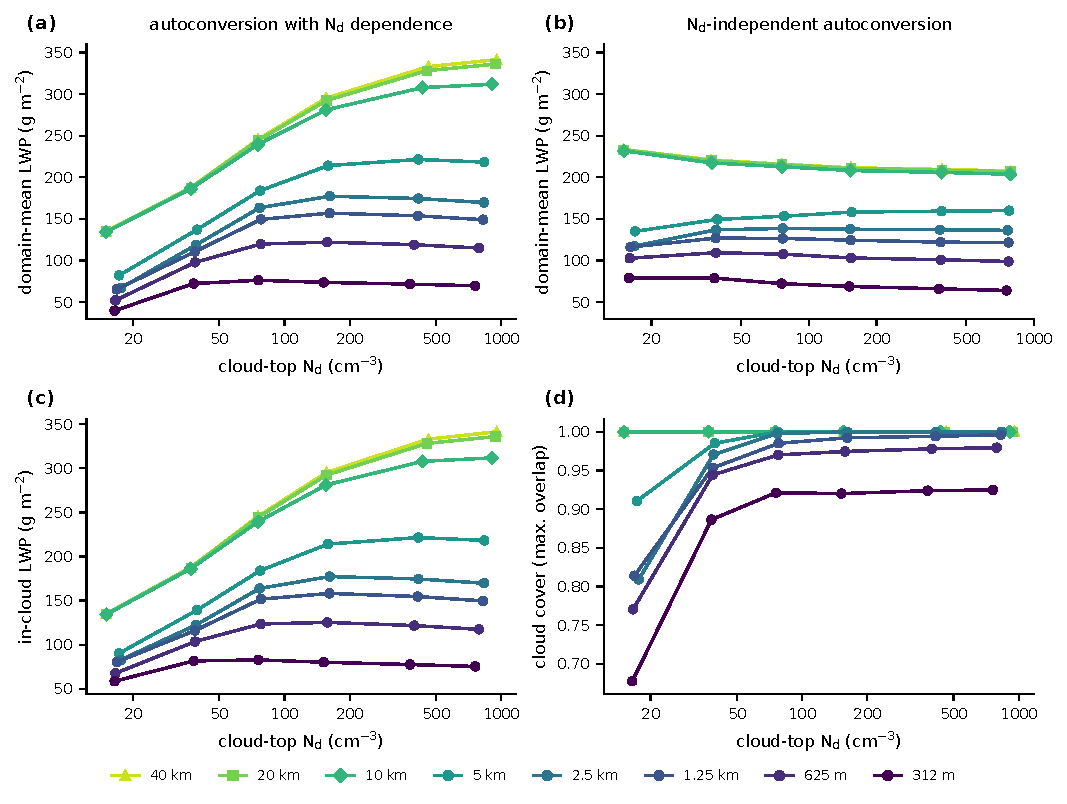
\includegraphics[width=\textwidth]{figures/fig03_response.pdf}
\caption{Response to cloud-top $\Nd$ at every grid spacing (sedimentation factor 1, hours 10--12). (a) Domain-mean LWP with $\Nd$-dependent and (b) $\Nd$-independent autoconversion. (c) In-cloud LWP and (d) maximum-overlap cloud cover with $\Nd$-dependent autoconversion.}\label{fig:response}
\end{figure}

\begin{figure}[t]
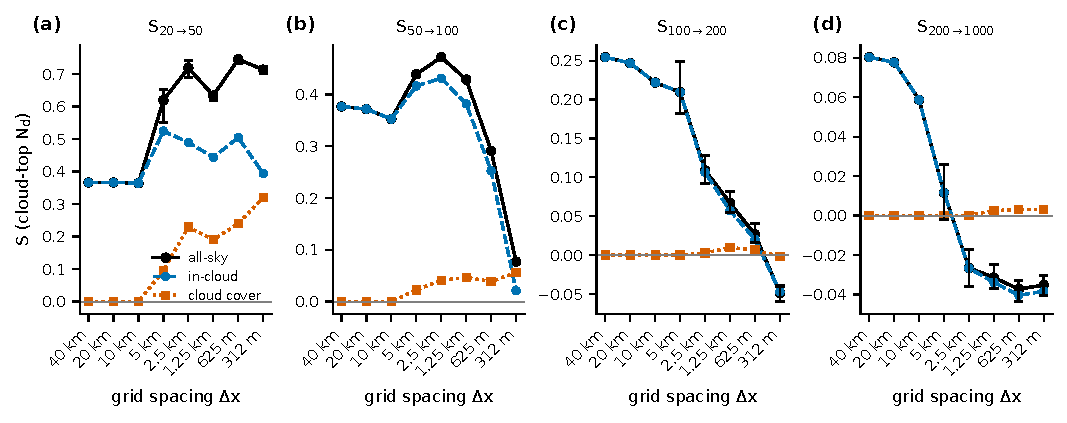
\includegraphics[width=\textwidth]{figures/fig04_Scomponents.pdf}
\caption{Susceptibility (cloud-top $\Nd$) on the four branches against grid spacing, split into in-cloud and cloud-cover parts (sedimentation factor 1, $\Nd$-dependent autoconversion, hours 10--12). Bars give the 5--95\,\% range of a 60\,km tile bootstrap ($\dx\leq5$\,km).}\label{fig:Scomp}
\end{figure}

\begin{table}[t]
\caption{Susceptibility with cloud-top $\Nd$ for sedimentation factor 1, hours 10--12. ``All'', ``ic'' and ``cc'' denote the all-sky value and its in-cloud and cloud-cover (maximum overlap) parts. ``Indep.'' denotes $\Nd$-independent autoconversion. $d\ln\tau/d\ln\Nd$ is for the moderate branch. $S_{55}$ is the local susceptibility at a cloud-top $\Nd$ of 55\,$\cmthree$ and $N_{0.1}$ the cloud-top $\Nd$ ($\cmthree$) above which $|S|<0.1$. Perturbed-twin and tile-bootstrap standard deviations are about 0.01 on the clean and moderate branches and 0.003 on the polluted branch at sub-kilometre spacing, and up to 0.03 at 5\,km.}\label{tab:S}
\begin{tabular}{lrrrrrrrrrrr}
\tophline
 & \multicolumn{3}{c}{$\Slow$} & \multicolumn{2}{c}{$\Shigh$} & $\Svhigh$ & \multicolumn{2}{c}{indep.} & & & \\
$\dx$ & all & ic & cc & all & ic & all & $\Shigh$ & $\Svhigh$ & $d\ln\tau/d\ln\Nd$ & $S_{55}$ & $N_{0.1}$ \\
\middlehline
40\,km & $0.37$ & $0.37$ & $0.00$ & $0.25$ & $0.25$ & $0.08$ & $-0.03$ & $-0.01$ & $0.55$ & 0.38 & 664 \\
20\,km & $0.37$ & $0.37$ & $0.00$ & $0.25$ & $0.25$ & $0.08$ & $-0.03$ & $-0.01$ & $0.54$ & 0.37 & 653 \\
10\,km & $0.36$ & $0.36$ & $0.00$ & $0.22$ & $0.22$ & $0.06$ & $-0.03$ & $-0.01$ & $0.52$ & 0.35 & 260 \\
5\,km & $0.62$ & $0.52$ & $0.10$ & $0.21$ & $0.21$ & $0.01$ & $0.05$ & $0.01$ & $0.51$ & 0.44 & 257 \\
2.5\,km & $0.72$ & $0.49$ & $0.23$ & $0.11$ & $0.11$ & $-0.03$ & $-0.01$ & $-0.01$ & $0.42$ & 0.47 & 259 \\
1.25\,km & $0.63$ & $0.44$ & $0.19$ & $0.07$ & $0.06$ & $-0.03$ & $-0.02$ & $-0.01$ & $0.38$ & 0.43 & 112 \\
625\,m & $0.75$ & $0.51$ & $0.24$ & $0.03$ & $0.02$ & $-0.04$ & $-0.06$ & $-0.03$ & $0.35$ & 0.29 & 111 \\
312\,m & $0.71$ & $0.39$ & $0.32$ & $-0.05$ & $-0.05$ & $-0.04$ & $-0.07$ & $-0.05$ & $0.29$ & 0.06 & 54 \\
\bottomhline

\end{tabular}
\end{table}

The radiative meaning of these susceptibilities differs from their sign. The optical-depth susceptibility $d\ln\tau/d\ln\Nd$ stays positive on every branch at every spacing. On the moderate branch it decreases from 0.55 at 40\,km to 0.29 at 312\,m, and on the clean branch it is 0.64 at 40\,km and 0.66--0.77 at finer spacing. In the offline albedo split, the LWP and cloud-cover terms amplify the Twomey term by 58\,\% at 40\,km on the moderate branch and offset it by 13\,\% at 312\,m, while on the clean branch they amplify it by 91\,\% at 40\,km and by a factor of 2.0--3.2 at $\dx\leq5$\,km, mostly through cloud cover. On the polluted branch the adjustment changes from $+16\,\%$ to between $-5$ and $-7\,\%$ of the Twomey term. The total potential albedo increase on the moderate branch is 0.079 at 40\,km and 0.046 at 312\,m. A change in the sign of the LWP susceptibility at high $\Nd$ therefore reduces the implied brightening without reversing it, whereas the clean-branch increase at fine spacing amplifies it. Because clean regimes dominate the uncertainty in aerosol forcing \citep{carslaw2013} and the cloud response to $\Nd$ is nonlinear \citep{jia2023}, the clean-branch result is the more relevant one for forcing estimates.

\subsection{Temporal evolution}\label{sec:time}

The resolution dependence develops during the simulations (Fig.~\ref{fig:time}). In hours 2--4, $\Shigh$ is 0.10--0.11 at every spacing from 40 to 2.5\,km and close to zero at $\dx\leq1.25$\,km; by hours 10--12 it has grown to 0.21--0.25 at 5--40\,km and has become negative at 312\,m, while at 1.25\,km and 625\,m it has increased slightly. The polluted branch is 0.04 at $\dx\geq2.5$\,km and $-0.01$ at finer spacing in hours 2--4, and it diverges in the same way. At 40\,km $S$ oscillates with periods of about 1.5--2\,h, so 2\,h averages are needed. The cloud-top $\Nd$ of the LWP maximum falls below the highest $\Nd$ level after about 3\,h at $\dx\leq1.25$\,km, after 5\,h at 2.5\,km and after about 9\,h at 5\,km, and at 312\,m it continues to decrease, from about 200 to 80\,$\cmthree$ between 5 and 12\,h. The inverted-V shape is thus time-dependent, and the statement that the maximum lies near 100\,$\cmthree$ at 312\,m refers to hour 12.

At $\dx\leq1.25$\,km, LWP decreases in nearly all runs throughout hours 4--12, and the coarse runs at high $\Nd$ are still thickening (by up to 15\,$\gmm$\,h$^{-1}$ at 40\,km), as in transient simulations of precipitating shallow convection \citep{seifert2015}. The phase plane of $d\LWP/dt$ against LWP at 312\,m (Fig.~\ref{fig:time}d) shows a common decline for all $\Nd$ that slows towards the end of the run. Exponential relaxation fits over hours 6--12 are well constrained only at 312\,m, where they give time scales of 4--7\,h and equilibrium LWP of about 45--55\,$\gmm$ for $\Nd\geq50\,\cmthree$, 25--35\,\% below the 12\,h values. At coarser spacing the fits do not constrain an equilibrium within 24\,h. The steady-state susceptibility at 312\,m implied by these fits, with 5--95\,\% intervals from a paired moving-block bootstrap, is $-0.11$ to $-0.21$ on the moderate branch in five of the six combinations of sedimentation and autoconversion setting (for $s=1$ and $\Nd$-dependent autoconversion $-0.13$, with an interval of $-0.23$ to $+0.06$), and $-0.17$ to $+0.06$ on the polluted branch. The negative moderate branch at 312\,m is therefore more likely to strengthen than to vanish as the runs approach equilibrium, while the sign of the polluted branch at equilibrium is undetermined. Fast and slow time scales coexist, as in mixed-layer and LES analyses \citep{bretherton2010,jones2014}, and the inversion is far from its equilibrium. With a subsidence time scale of 74\,h, $\we/D$ is about 1000\,m at 40\,km and about 2200\,m at 312\,m, compared with $\zi$ of 860 and 1020\,m at 12\,h. A susceptibility of about $-0.05$ after 11\,h is weaker than the LWP adjustments found after a similar time in an LES ensemble of non-precipitating nocturnal stratocumulus \citep{chen2025}.

\begin{figure}[t]
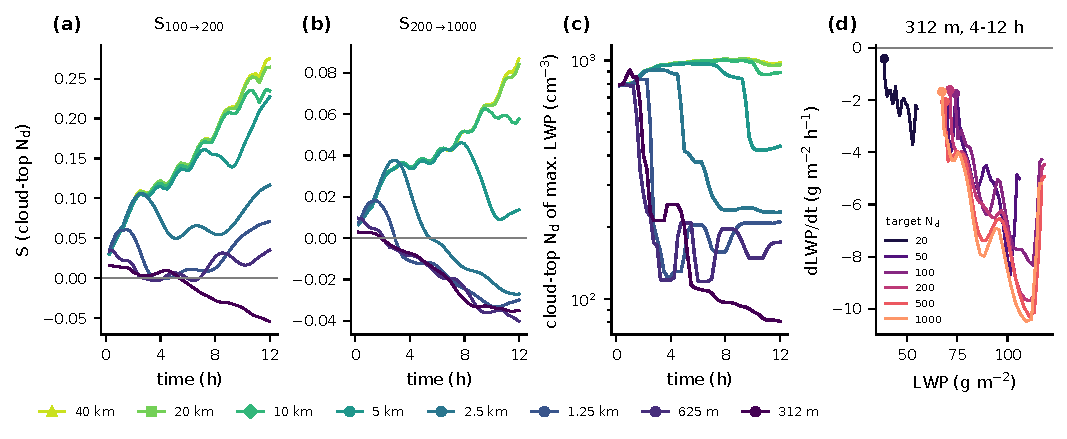
\includegraphics[width=\textwidth]{figures/fig05_time.pdf}
\caption{Temporal evolution ($\Nd$-dependent autoconversion, sedimentation factor 1). (a) $\Shigh$ and (b) $\Svhigh$ from 15\,min output (2\,h running mean). (c) Cloud-top $\Nd$ of the LWP maximum (2\,h running median); values near the top of the axis indicate a maximum at the highest $\Nd$ level. (d) Phase plane of $d\LWP/dt$ against LWP at 312\,m for hours 4--12; dots mark hour 12.}\label{fig:time}
\end{figure}

\subsection{Susceptibility and the base-state regime}\label{sec:regime}

Figure~\ref{fig:regime} plots $S$ against the precipitation-to-entrainment-drying ratio of the lower-$\Nd$ run for all grid spacings, sedimentation factors and both autoconversion settings. With $\Nd$-dependent autoconversion, $\Shigh$ follows this ratio closely across the 24 combinations of grid spacing and sedimentation factor (correlation 0.92). The ratio alone explains 84\,\% of the variance of $\Shigh$, and adding $\log\dx$ as a second predictor raises this only to 86\,\%. This also explains why $\Shigh$ increases with $s$ at 2.5 and 1.25\,km, because faster sedimentation raises the base-state surface precipitation there and moves the runs along the same curve. On the middle branch the correlation is 0.70, and on the polluted branch 0.75, where grid spacing retains additional explanatory power (variance explained 57\,\% by the ratio alone and 85\,\% with $\log\dx$), consistent with the change in entrainment efficiency at constant, nearly zero precipitation. With $\Nd$-independent autoconversion the relationship is weaker (correlations 0.45--0.65) and $S$ is near zero over most of the range. On the clean branch the ratio has no explanatory power, because the response there is dominated by cloud cover at fine spacing.

\begin{figure}[t]
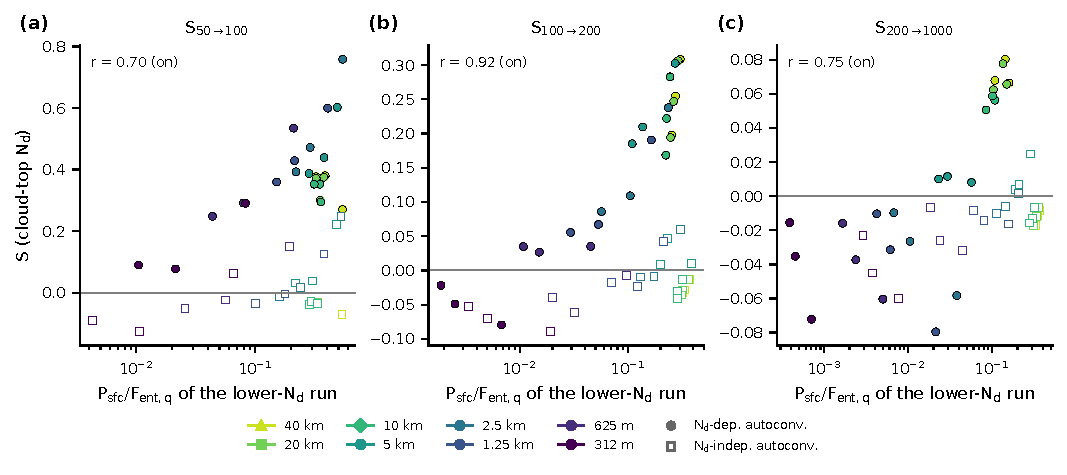
\includegraphics[width=\textwidth]{figures/fig06_regime.pdf}
\caption{Susceptibility (cloud-top $\Nd$, hours 10--12) against the ratio of surface precipitation to entrainment drying of the lower-$\Nd$ run, for all grid spacings and sedimentation factors, on the (a) middle, (b) moderate and (c) polluted branches. Filled circles: $\Nd$-dependent autoconversion; open squares: $\Nd$-independent. Correlations refer to $\Nd$-dependent autoconversion.}\label{fig:regime}
\end{figure}

The base state changes with grid spacing because the coarse and fine clouds differ in depth, base height and turbulence. Rain production at target 200\,$\cmthree$ decreases from 0.55\,mm\,d$^{-1}$ at 40\,km to 0.03\,mm\,d$^{-1}$ at 312\,m as the cloud thins from about 650 to 300\,m, and the fraction that evaporates below cloud base increases from 0.40 to 0.93 (Fig.~\ref{fig:rain}). Meanwhile the entrainment drying flux roughly doubles, from 67 to 128\,W\,m$^{-2}$, so the ratio of surface precipitation to entrainment drying decreases by a factor of about 300 at targets 200--1000\,$\cmthree$ and of about 4 at target 20\,$\cmthree$. Resolved variability partly compensates for the thinner cloud, since the autoconversion enhancement $\langle q_\mathrm{c}^{2.47}\rangle/\langle q_\mathrm{c}\rangle^{2.47}$ is 1.00 at $\dx\geq10$\,km, 1.1--1.3 at $\dx\leq5$\,km and target $\Nd\geq200\,\cmthree$, and 1.4--1.9 at target 20\,$\cmthree$. The precipitation susceptibility $S_R$ on the moderate branch increases from 0.9 at 40\,km to 2.4--2.8 at $\dx\leq2.5$\,km, the coarse value reflecting the light, ubiquitous drizzle of the single-column limit (raining fraction 1.0 at target 20--50\,$\cmthree$), which resembles the frequent light rain of GCMs \citep{michibata2016,mulmenstadt2020}. When surface precipitation is negligible, precipitation suppression has little effect on LWP, and the decrease of LWP with $\Nd$ associated with entrainment dominates \citep{ackerman2004,wood2007,hoffmann2020}; in EAMxx, grid spacing determines which of these regimes the simulated cloud occupies.

\begin{figure}[t]
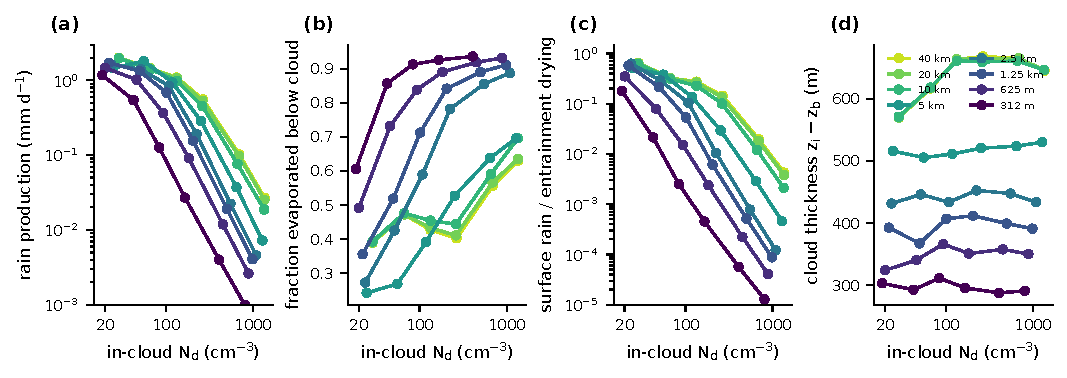
\includegraphics[width=\textwidth]{figures/fig07_rain.pdf}
\caption{Precipitation against in-cloud $\Nd$ at every grid spacing ($\Nd$-dependent autoconversion, sedimentation factor 1). (a) Column rain production. (b) Fraction of the production that evaporates before reaching the surface. (c) Ratio of surface precipitation to entrainment drying. (d) Cloud thickness $\zi-\zb$.}\label{fig:rain}
\end{figure}

\subsection{Drizzle, sedimentation and entrainment}\label{sec:sed}

Switching off the $\Nd$ dependence of autoconversion changes LWP through two parts of opposite sign, a rain sink and a drizzle effect on entrainment. In the mixed-layer budget at target $\Nd\geq200\,\cmthree$, removing the heavy drizzle of the $\Nd$-independent runs (that is, the difference between the two autoconversion settings) contributes $+4$ to $+6$\,\%\,h$^{-1}$ through the precipitation term at $\dx\geq5$\,km, but only $+0.2$ to $+1$\,\%\,h$^{-1}$ at 625 and 312\,m. At the same time it raises $\we$ by 0.2\,mm\,s$^{-1}$ at 20--40\,km and by up to 1.4\,mm\,s$^{-1}$ at $\dx\leq2.5$\,km (Fig.~\ref{fig:entrain}b), consistent with drizzle stabilising the subcloud layer and reducing entrainment \citep{stevens1998,ackerman2009}. The difference between the two autoconversion settings therefore measures the precipitation-suppression effect net of a drizzle--entrainment effect, and its small value at fine spacing partly reflects cancellation. The factorial decomposition of Appendix~\ref{app:decomp} shows in addition that the effect of sedimentation on $S$ at coarse spacing depends on the autoconversion formulation, and that the partition between precipitation and sedimentation terms depends on the matching $\Nd$ of the $\Nd$-independent configuration.

The offline cloud-top sedimentation flux at $s=1$ is 0.4--1.5\,mm\,d$^{-1}$, with mass-weighted fall speeds of 1.0--1.2\,cm\,s$^{-1}$ at target 1000\,$\cmthree$, 1.8--2.3\,cm\,s$^{-1}$ at 200\,$\cmthree$ and 3.8--5.3\,cm\,s$^{-1}$ at 20\,$\cmthree$. Increasing $s$ from 0.5 to 2 raises this flux by 0.5--1.5\,mm\,d$^{-1}$ at target $\Nd\geq200\,\cmthree$ at all grid spacings (Fig.~\ref{fig:entrain}a). At $\dx\leq2.5$\,km this increase is accompanied by a decrease of $\we$ by 0.2--1.2\,mm\,s$^{-1}$ (regression slope $-0.8$\,mm\,s$^{-1}$ per mm\,d$^{-1}$, correlation $-0.31$), whereas at $\dx\geq10$\,km $\we$ does not respond (slope $-0.03$). The sedimentation--entrainment coupling of \citet{bretherton2007} thus operates at $\dx\leq2.5$\,km and is absent at coarse spacing, where the inversion is pinned. At low $\Nd$ the larger decrease of $\we$ with $s$ (1.1--2.4\,mm\,s$^{-1}$ at $\dx\leq5$\,km) occurs together with large fall speeds and drizzle, so it is not a clean measure of the sedimentation--entrainment coupling. Because P3 sedimentation acts after SHOC's adjustment within each step and the cloud-top fields are written after P3, the time step (100\,s at coarse and 15\,s at fine spacing) may also affect how much cloud-top liquid is removed per step; cloud-top $\Nd$ relative to the target decreases with $s$ by 8--12\,\% at 40\,km but not at 312\,m.

\begin{figure}[t]
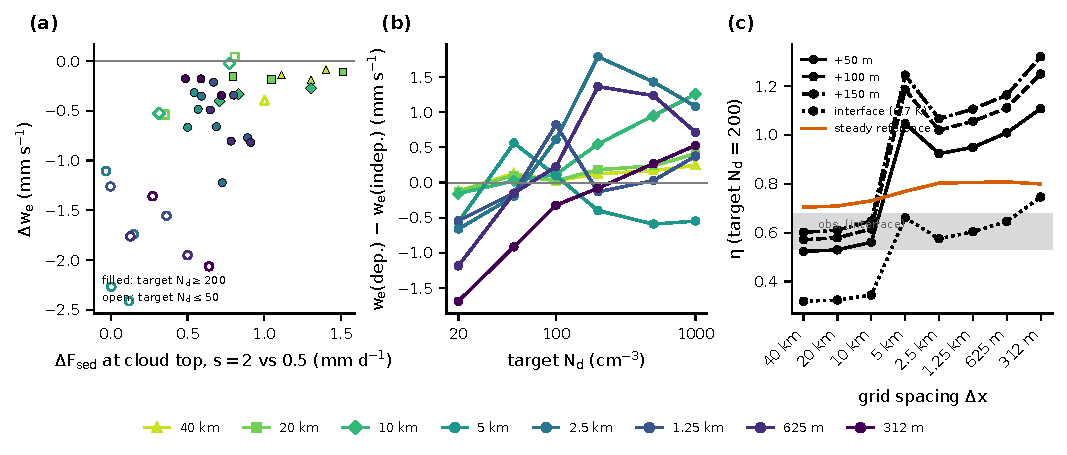
\includegraphics[width=\textwidth]{figures/fig08_entrainment.pdf}
\caption{(a) Change in entrainment rate against change in the offline cloud-top sedimentation flux between sedimentation factors 2 and 0.5 ($\Nd$-dependent autoconversion); filled symbols target $\Nd\geq200\,\cmthree$, open symbols $\leq50\,\cmthree$. (b) Difference in entrainment rate between $\Nd$-dependent and $\Nd$-independent autoconversion (sedimentation factor 1). (c) $\eta$ at target $\Nd=200\,\cmthree$ for jumps taken 50, 100 and 150\,m above $\zi$ and for the specified interface jump, with the steady-state reference and the observed range for the interface definition.}\label{fig:entrain}
\end{figure}

\subsection{Decoupling and the mixed-layer budget}\label{sec:budget}

The degree of coupling depends on the metric (Fig.~\ref{fig:decoup}). The coarse runs have the largest moisture difference across the boundary layer ($\Delta q_t=1.1$--1.5\,g\,kg$^{-1}$), produced by SHOC's down-gradient transport of the surface moisture flux, but their $\theta_l$ is well mixed, the buoyancy flux below cloud base stays at 40--110\,\% of its surface value and cloud base lies within 35\,m of the mixed-layer condensation level, so they are coupled by the Jones test and by the flux criterion. At 312\,m and target $\Nd\geq100\,\cmthree$, $\Delta q_t$ is only 0.2--0.3\,g\,kg$^{-1}$, but the buoyancy-flux minimum below cloud base is 8--10\,\% of the surface value, cloud base lies 50--70\,m above the mixed-layer condensation level, and the variance is concentrated below cloud. Refinement therefore increases decoupling by the buoyancy-flux and cloud-base metrics while decreasing it by $\Delta q_t$. The buoyancy flux is not significantly negative below cloud base in any run, so the low-$\Nd$ states resemble cumulus rising into stratocumulus, without a stable subcloud layer.

\begin{figure}[t]
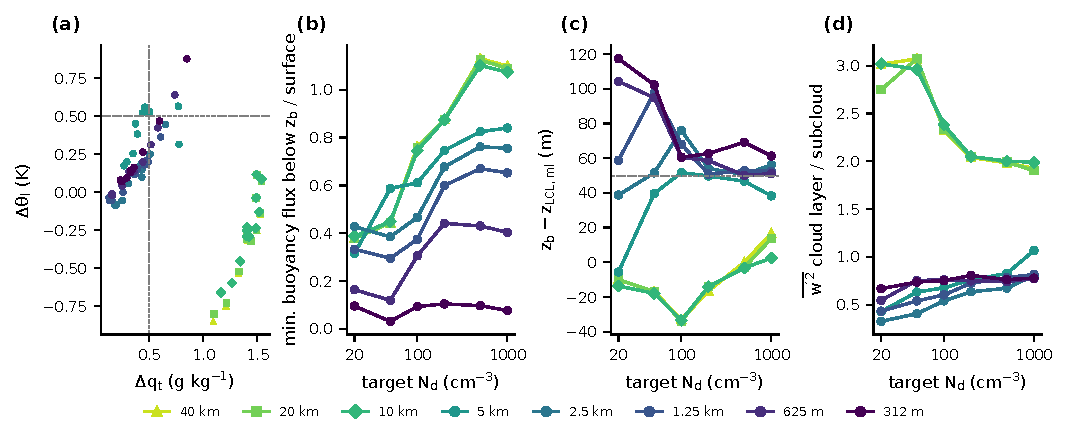
\includegraphics[width=\textwidth]{figures/fig10_decoupling.pdf}
\caption{Decoupling metrics (sedimentation factor 1, hours 10--12). (a) $\Delta\theta_l$ against $\Delta q_t$ between the highest and lowest quarters of the layer below the inversion base for both autoconversion settings, with the thresholds of \citet{jones2011}. (b) Minimum total buoyancy flux below cloud base relative to the surface value, (c) cloud base above the mixed-layer lifting condensation level, and (d) ratio of cloud-layer to subcloud vertical-velocity variance, for $\Nd$-dependent autoconversion.}\label{fig:decoup}
\end{figure}

By the combined criterion of Sect.~\ref{sec:mlb}, 97\,\% of the 2\,h windows at $\dx\geq10$\,km are coupled, 58\,\% at 5\,km, 11\,\% at 2.5\,km and at most 3\,\% at $\dx\leq1.25$\,km. The mixed-layer budget (Fig.~\ref{fig:budget}) is therefore used for attribution only at coarse spacing. There it reproduces the in-cloud LWP tendency in coupled windows with correlations of 0.72--0.76, and the increase of LWP with $\Nd$ at 40\,km follows from the removal of the precipitation sink ($-10$\,\%\,h$^{-1}$ at target 20\,$\cmthree$ and nearly zero at $\geq500\,\cmthree$) at an entrainment contribution that is constant in $\Nd$. At 2.5\,km and finer the correlation for in-cloud LWP falls to 0.47 and 0.07--0.32, and the entrainment contribution splits into a deepening part of $+10$ to $+20$\,\%\,h$^{-1}$ and a cloud-base part of $-30$ to $-50$\,\%\,h$^{-1}$ at 312\,m, so the net thinning is the small difference of large terms in a decoupled layer. The budget is consistent with the view that stronger entrainment raises cloud base faster than it deepens the layer at fine spacing, but it does not establish which process sets the small negative susceptibilities there.

\begin{figure}[t]
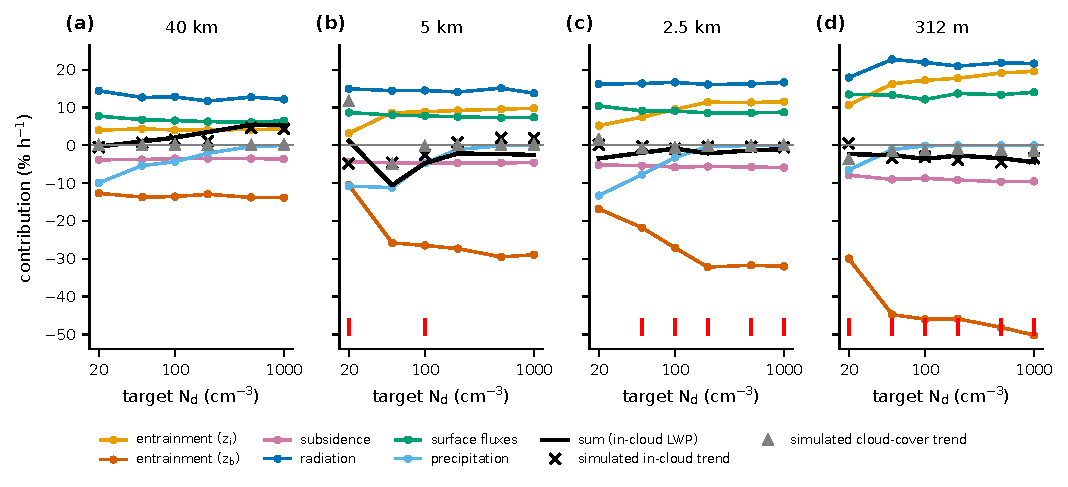
\includegraphics[width=\textwidth]{figures/fig09_budget.pdf}
\caption{Mixed-layer budget of in-cloud LWP for hours 10--12 at (a) 40\,km, (b) 5\,km, (c) 2.5\,km and (d) 312\,m ($\Nd$-dependent autoconversion, sedimentation factor 1), with the entrainment term split into deepening and cloud-base parts. Crosses and triangles are the simulated tendencies of in-cloud LWP and cloud cover. Red ticks mark windows that fail the coupling criterion, for which the attribution is not valid.}\label{fig:budget}
\end{figure}

\subsection{Robustness}\label{sec:robust}

The perturbed twins give standard deviations of the differences in $S$ of 0.007--0.010 on the clean, middle and moderate branches and 0.002--0.004 on the polluted branch at 625 and 312\,m, so a single run has a noise of about 0.007 and 0.002, respectively. The tile bootstrap gives similar values at sub-kilometre spacing (0.006 and 0.003) and up to 0.03 at 5\,km. The moderate-branch value at 312\,m ($-0.05$, negative for all three sedimentation factors and both autoconversion settings) and the polluted-branch values at $\dx\leq2.5$\,km are therefore well outside the internal noise. The moderate branch at 625\,m (0.03) changes sign with the autoconversion setting, and the location of the LWP maximum is not resolvable. The main threats to the fine-grid results are thus transience (Sect.~\ref{sec:time}) and structural choices, in particular the fixed vertical grid and the mixing-length cap, rather than internal variability. The 3D-turbulence option changes LWP by less than 1.5\,\% and $\we$ by less than 0.13\,mm\,s$^{-1}$ (Appendix~\ref{app:t3d}).

%% ====================================================================
\section{Discussion}\label{sec:discussion}
%% ====================================================================

\subsection{One mixed-layer argument}

The results can be summarised by a single chain. Grid spacing changes the entrainment rate (Sect.~\ref{sec:regimes}); the entrainment rate sets the depth and base height of the cloud and hence its rain production and the fraction of rain that evaporates (Sect.~\ref{sec:regime}); and the resulting ratio of precipitation to entrainment drying sets the moderate-branch susceptibility, as in the mixed-layer arguments of \citet{ackerman2004}, \citet{wood2007} and \citet{hoffmann2020}. At coarse spacing the sink removed by precipitation suppression is large and the response is positive; at fine spacing there is little rain to suppress, the sedimentation--entrainment coupling becomes active and the response is near zero or slightly negative. Most of the resolution dependence of $\Shigh$ is thus a dependence on the simulated cloud regime, which grid spacing controls in EAMxx; at fixed regime, grid spacing adds little explanatory power on this branch. The near-zero susceptibility at fine spacing reflects an absent precipitation sink, which differs from the compensation between processes that \citet{stevens2009} described as buffering. Two parts of the response do not follow this chain, namely the cloud-cover response on the clean branch, which is absent at coarse spacing by construction and which dominates the radiative relevance at fine spacing, and the polluted branch, which retains a dependence on grid spacing at nearly zero precipitation.

The first link of the chain is the least physical. Entrainment changes abruptly between 10 and 5\,km as the 5\,km runs leave a state pinned at the inversion, and at 5\,km the resolved flow is dominated by near-grid-scale motions. At $\dx\leq2.5$\,km about half of the inferred entrainment flux is not carried by resolved or parameterised turbulence, the inversion spans two to three levels and cloud-top height varies by less than one level. LES studies show that entrainment converges from above as the inversion is resolved \citep{stevens1999res,stevens2005,pressel2017,mellado2018}. Our sub-kilometre runs, with fixed 50\,m levels, a capped mixing length and an entrainment efficiency of 2.0--2.6 at 312\,m, are therefore unlikely to lie on a path towards the LES solution, and a converged answer probably requires entrainment to decrease again with vertical refinement. The grey zone for stratocumulus in EAMxx with SHOC begins at about 5\,km, and remedies would include scale-aware partitioning of turbulence \citep{boutle2014,efstathiou2015,honnert2011} and vertical resolution at the inversion consistent with the horizontal grid \citep{bogenschutz2023rrm}.

\subsection{Relation to other models and to LES}

The coarse configuration reproduces features of GCM behaviour, namely no cloud-cover response, light ubiquitous drizzle and a positive response driven by autoconversion, although with a 100\,s time step and 50\,m levels it is not a GCM column. The comparison with \citet{mulmenstadt2024adj}, who found an active sedimentation--entrainment coupling in E3SM single-column physics, indicates that whether this coupling appears in single-column physics depends on the turbulence scheme and its vertical representation of the inversion, which is pinned at a model level in our coarse runs. \citet{terai2020} found weaker LWP increases at 250\,m than at 4\,km in a multiscale model because of weaker increases in non-raining clouds and a smaller raining fraction, the same tendency as in our runs. \citet{sato2018} attributed LWP decreases in a global cloud-system-resolving model to explicitly simulated condensation and evaporation, a pathway absent from EAMxx. The 312\,m polluted-branch value after 11\,h ($-0.04$) is of a similar magnitude to the weak nocturnal LWP decreases at high $\Nd$ in LES by \citet{hill2009} and to the weak slopes expected for weakly and non-precipitating stratocumulus by \citet{hoffmann2025}, and weaker than the LES ensemble of \citet{chen2025} at a similar time after perturbation. Possible reasons include the absence of a size-dependent evaporation--entrainment effect in SHOC \citep{wang2003,hoffmann2019}, the 50\,m levels, drizzle at the lower $\Nd$ levels, and the moderately humid free troposphere of RF02 ($\Delta q_t$ of 5.8--6.5\,g\,kg$^{-1}$ at the inversion). Because solar heating buffers the nocturnal decline of LWP \citep{zhang2024,chen2024,sandu2008} and the meteorological controls on albedo susceptibility differ between regions and times of day \citep{zhang2019,zhang2023}, a diurnally averaged susceptibility cannot be inferred from these runs, and the nocturnal values are likely to overstate the thinning.

Satellite-style analyses of these simulations are hypothetical because the case is nocturnal; they are summarised in Appendix~\ref{app:sat}. With horizontally uniform CCN, within-scene variability accounts for less than 1\,\% of the variance of cloud-top $\ln\Nd$, so pooled composites reproduce the between-run slope, whereas a retrieval-like adiabatic $\Nd$ is about twice the model value and half of its variance is within-scene noise correlated with LWP, which lowers the pooled slope substantially. Selecting overcast, non-raining columns alone shifts the slope by up to 0.1. These results are consistent with \citet{gryspeerdt2019}, \citet{quaas2020}, \citet{arola2022}, \citet{gryspeerdt2022amt} and \citet{kokkola2025}, and with large-domain LES analyses of satellite-style relationships \citep{costasuros2020,dipu2022}, and they do not add a separate conclusion.

\subsection{Limitations and future experiments}\label{sec:limits}

The study simulates one nocturnal, drizzling case with constant forcing, and hours 10--12 have no counterpart in nature. Each configuration was run once with a common initial perturbation; the perturbed twins bound the internal noise but not the structural uncertainty. After 12\,h the sub-kilometre runs are still adjusting, and the steady-state values depend on exponential extrapolation. The vertical grid was fixed, SHOC's mixing length was capped at the grid spacing, the time step co-varied with grid spacing, the radiation scheme lacks the above-inversion balancing term of the protocol, and the absence of Coriolis force and wind nudging allowed the shear to decay. CCN were prescribed and uniform, without aerosol processing \citep{kazil2011,berner2013,goren2019,yamaguchi2017}, condensation was diagnosed by saturation adjustment, and autoconversion followed KK2000 without subgrid enhancement. The decomposition into precipitation and sedimentation terms depends on the matching $\Nd$ of the $\Nd$-independent configuration and on an extrapolation in $s$. The most informative future experiments would be a paired-perturbation design in which the runs are spun up at a common $\Nd$ and then perturbed and integrated for 24--36\,h with several seeds; a 312\,m pair with 10--15\,m levels near the inversion; a 36\,h set with a diurnal cycle; simulations with a sedimentation factor of zero and with a second matching $\Nd$ for the $\Nd$-independent configuration; tests with a common time step and a relaxed mixing-length cap; and an LES reference with the same microphysics.

%% ====================================================================
\conclusions\label{sec:conclusions}
%% ====================================================================

We analysed 288 doubly periodic EAMxx simulations of the nocturnal, drizzling DYCOMS-II RF02 stratocumulus under constant forcing, with grid spacings from 40\,km to 312\,m, six $\Nd$ levels, three sedimentation factors and two autoconversion settings. Our conclusions are as follows.
\begin{enumerate}
\item After 10--12\,h, the moderate-branch LWP susceptibility decreased from 0.25 at 40\,km to $-0.05$ at 312\,m and the polluted branch became weakly negative at $\dx\leq2.5$\,km (23 of 24 configurations), whereas the clean-branch susceptibility increased from 0.37 to 0.62--0.75, largely through cloud cover. The optical-depth susceptibility stayed positive, so the implied brightening is reduced at high $\Nd$ and amplified at low $\Nd$ at fine spacing.
\item The moderate-branch susceptibility tracks the ratio of surface precipitation to entrainment drying of the base state across grid spacings and sedimentation factors. In EAMxx, grid spacing acts mainly by setting the cloud regime through the entrainment rate, which determines cloud depth, cloud base, rain production and subcloud evaporation.
\item The resolution dependence develops over the run and the fine-grid runs are still adjusting. The 312\,m moderate-branch value is well outside the internal noise and more likely to strengthen than to vanish at equilibrium, whereas the equilibrium sign of the polluted branch is undetermined.
\item Part of the increase of entrainment with refinement is implicit mixing at an inversion spanning two to three 50\,m levels, the 5\,km runs are dominated by near-grid-scale circulations, and the 312\,m runs do not approximate LES. Extending these results to physical estimates requires vertical refinement at the inversion, longer and diurnally forced simulations, and paired-perturbation ensembles.
\end{enumerate}

%% ====================================================================
\appendix
%% ====================================================================

\section{Factorial decomposition}\label{app:decomp}

For each grid spacing and branch we fitted $S_\mathrm{dep}(s)=a_\mathrm{dep}+b_\mathrm{dep}s$ and $S_\mathrm{ind}(s)=a_\mathrm{ind}+b_\mathrm{ind}s$ for $\Nd$-dependent and $\Nd$-independent autoconversion over $s=0.5$, 1 and 2, and decomposed $S_\mathrm{dep}(1)=(a_\mathrm{dep}-a_\mathrm{ind})+b_\mathrm{ind}+(b_\mathrm{dep}-b_\mathrm{ind})+a_\mathrm{ind}$ into an autoconversion term at zero sedimentation, a sedimentation term, an interaction and a residual (Fig.~\ref{fig:decompA}, computed with the layer $\Nd$ of the first version). At $\dx\geq10$\,km the autoconversion term on the moderate branch is 0.34--0.39 and the interaction $-0.07$ to $-0.08$, because $\Shigh$ decreases strongly with $s$ only with $\Nd$-dependent autoconversion; at finer spacing the autoconversion term decreases to 0.04--0.12. Because the $\Nd$-independent runs drizzle heavily at high $\Nd$, the extrapolation to $s=0$ has one residual degree of freedom and $S$ is convex in $s$ on the clean branch, the partition depends on the design and should not be read as a pivot-independent attribution. Section~\ref{sec:regime} offers a simpler interpretation, in which sedimentation moves the base state along the regime curve.

\begin{figure}[t]
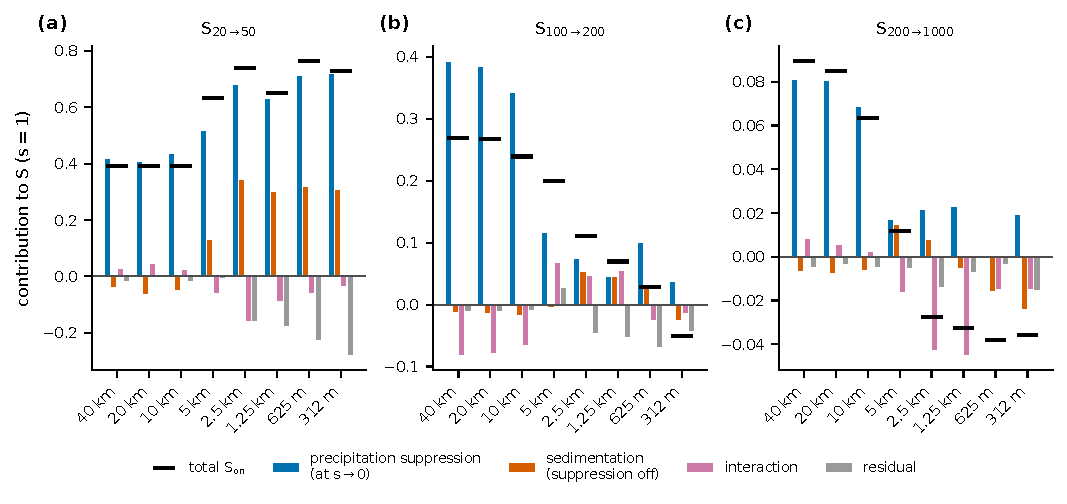
\includegraphics[width=\textwidth]{figures/figA1_decomposition.pdf}
\caption{Factorial decomposition of the susceptibility with $\Nd$-dependent autoconversion at sedimentation factor 1 (black bars) on the (a) clean, (b) moderate and (c) polluted branches.}\label{fig:decompA}
\end{figure}

\section{SHOC mixing length and activation floor}\label{app:shoc}

Figure~\ref{fig:shocmix}a shows the domain-mean SHOC mixing length at target 200\,$\cmthree$. At $\dx\geq10$\,km it reaches about 1600\,m near 0.85\,$\zi$, about twice the boundary-layer depth, because the grid-length cap is not active. At 5\,km to 1.25\,km it peaks at 900--1100\,m and is 600--800\,m below. At 625\,m it is 480--610\,m, close to the cap, and at 312\,m it equals the cap nearly everywhere in the boundary layer. Figure~\ref{fig:shocmix}b shows that the in-cloud $\Nd$ follows the activation floor, which decreases with height; between 6 and 12\,h the layer $\Nd$ decreases by about 3\,\%\,h$^{-1}$ at $\dx\leq625$\,m as the cloud rises into air with less CCN.

\begin{figure}[t]
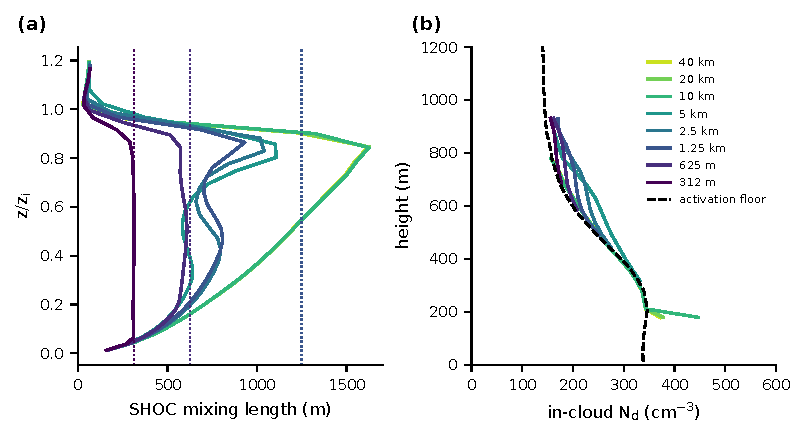
\includegraphics[width=0.75\textwidth]{figures/figA3_shocmix_nd.pdf}
\caption{(a) Domain-mean SHOC mixing length against $z/\zi$ and (b) in-cloud $\Nd$ with the activation floor (dashed), for target $\Nd=200\,\cmthree$, hours 10--12, $\Nd$-dependent autoconversion and sedimentation factor 1. Dotted lines in (a) mark the grid-spacing cap at 1.25\,km, 625\,m and 312\,m.}\label{fig:shocmix}
\end{figure}

\section{3D turbulence twins}\label{app:t3d}

Figure~\ref{fig:t3d} shows the differences between the 71 runs with 3D turbulence on and their partners. LWP changes by between $-1.0$ and $+1.4\,\gmm$, cloud cover by between $-0.005$ and $+0.007$, and the entrainment rate by between $-0.13$ and $+0.02$\,mm\,s$^{-1}$; the root-mean-square relative LWP difference in hours 10--12 is 0.6\,\%.

\begin{figure}[t]
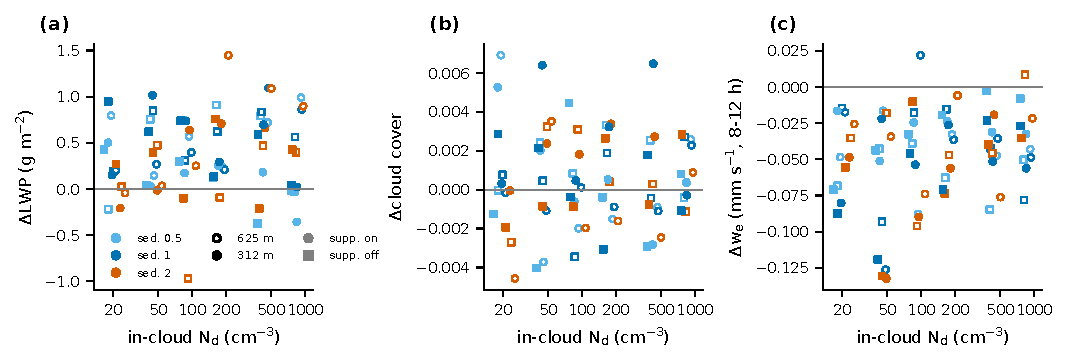
\includegraphics[width=\textwidth]{figures/figA4_turb3d.pdf}
\caption{Difference (3D turbulence on minus off) in (a) LWP, (b) cloud cover (LWP above 10\,$\gmm$) and (c) entrainment rate at 625\,m (open symbols) and 312\,m (filled symbols), coloured by sedimentation factor; circles: $\Nd$-dependent, squares: $\Nd$-independent autoconversion.}\label{fig:t3d}
\end{figure}

\section{LWP spectra and distributions}\label{app:spectra}

The LWP spectral peak (Fig.~\ref{fig:spectra}) lies at 48\,km at 5\,km and about 30\,km at 2.5\,km, 6.4 and 8 physics-column spacings, which suggests that it is limited by the effective resolution of the dynamical core, and at 13--22\,km at 625 and 312\,m, an aspect ratio of 13--20 that is on the narrow side of observed closed cells \citep{wood2006,glassmeier2017}. Pockets of open cells were observed during RF02 and in LES of the case \citep{stevens2005poc,savicjovcic2008}, so the broken low-$\Nd$ fields are plausible, whereas the reduced cloud cover at high $\Nd$ at 312\,m has no observational counterpart in this case.

\begin{figure}[t]
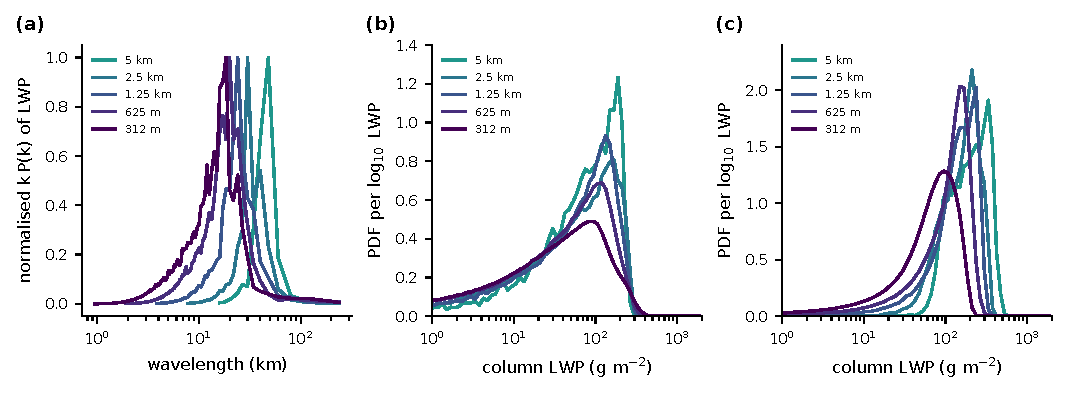
\includegraphics[width=\textwidth]{figures/figA5_spectra_pdf.pdf}
\caption{(a) Normalised radially averaged LWP spectra (hours 10--12) for target $\Nd=200\,\cmthree$. (b, c) Distributions of column LWP over hours 10--12 for target $\Nd$ of 20 and 1000\,$\cmthree$. $\Nd$-dependent autoconversion, sedimentation factor 1.}\label{fig:spectra}
\end{figure}

\section{Satellite-style analysis}\label{app:sat}

To illustrate how satellite-style estimators would perform if these clouds could be observed, we pooled the cloudy columns of the six $\Nd$ runs at each grid spacing with equal weight per run and computed the regression of column $\ln\LWP$ on column $\ln\Nd$ (Fig.~\ref{fig:sat}). Columns were selected with a satellite-like filter: cloud-top liquid fraction above 0.9, LWP above 20\,$\gmm$, cloud-top effective radius below 15\,$\mu$m and optical depth above 3. The retrieval-like $\Nd$ follows the adiabatic formula of \citet{grosvenor2018} applied to column LWP and cloud-top effective radius, at native resolution and after averaging to a common 3.75\,km scale \citep{mccomiskey2012}. With model cloud-top $\Nd$, the within-scene share of the $\ln\Nd$ variance is below 1\,\% (within-scene standard deviation of $\ln\Nd$ at most 0.12, correlations between $-0.66$ and $+0.57$), so the pooled slope (0.10 at 312\,m to 0.27 at 5\,km) equals the between-run slope; it exceeds the slope of in-cloud LWP for all columns (0.00 to 0.19) because the filter removes broken and drizzling columns. With retrieval-like $\Nd$, which is about twice the model value, the within-scene share is 46--52\,\% and the pooled slope (0.04--0.23) is only 25--50\,\% of the between-run slope (0.13--0.46), illustrating the dilution and bias by retrieval errors correlated with LWP \citep{jia2019,arola2022,kokkola2025,jia2022}. Because activation in EAMxx does not depend on updraft speed, the model lacks the updraft-driven covariation of $\Nd$ and LWP found in nature, and the within-scene relationships should not be generalised to observations.

\begin{figure}[t]
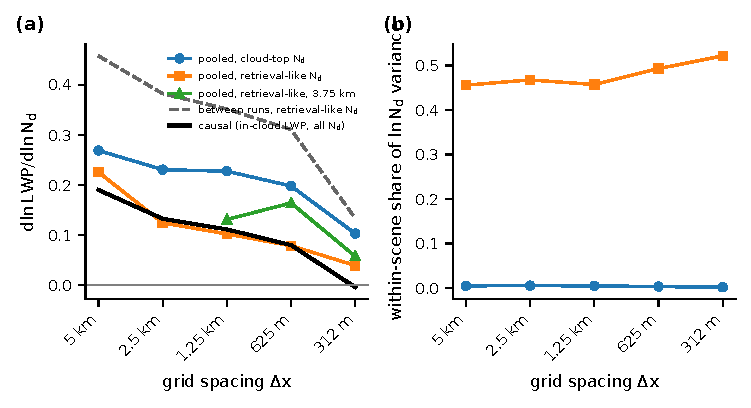
\includegraphics[width=0.7\textwidth]{figures/figA6_satellite.pdf}
\caption{(a) Pooled-composite slope of $\ln\LWP$ on $\ln\Nd$ for cloud-top $\Nd$ and retrieval-like $\Nd$ (native and 3.75\,km), the between-run slope with retrieval-like $\Nd$, and the slope of in-cloud LWP for all columns ($\Nd$-dependent autoconversion, sedimentation factor 1, hours 10--12). (b) Within-scene share of the pooled $\ln\Nd$ variance.}\label{fig:sat}
\end{figure}

\noappendix

%% ====================================================================
\codedataavailability{\sloppy The model code is the E3SM branch \texttt{mahf708/eamxx/p3-cloud-sed-factor} at \url{https://github.com/mahf708/E3SM/tree/mahf708/eamxx/p3-cloud-sed-factor}, which contains E3SM pull request 9017 (the cloud-top output operator) and the P3 sedimentation-factor option. Run scripts and all analysis scripts used to produce the tables and figures are in the \texttt{sed-precsupp-study} directory of the branch \url{https://github.com/mahf708/scmlib/tree/sed-precsupp-study}. Model output and the derived tables are available from the corresponding contact on request.}

\authorcontribution{Naser Mahfouz and Johannes M\"ulmenst\"adt designed the experiments, and Naser Mahfouz implemented the model modifications and performed the simulations. The author, an AI system (Claude, Anthropic), designed and carried out the analysis and wrote the manuscript at the direction of Naser Mahfouz and Johannes M\"ulmenst\"adt. Human review of the manuscript is pending.}

\competinginterests{The author declares that there are no competing interests.}

\begin{acknowledgements}
Naser Mahfouz and Johannes M\"ulmenst\"adt (Pacific Northwest National Laboratory) designed and directed this study, and Naser Mahfouz is the contact person for correspondence. The simulations used the Energy Exascale Earth System Model (E3SM) and resources of the National Energy Research Scientific Computing Center (NERSC), a U.S. Department of Energy Office of Science User Facility, on the Perlmutter system. The analysis and the text were produced by an AI system (Claude, Anthropic); all analysis scripts are provided so that the results can be verified.
\end{acknowledgements}

\bibliographystyle{copernicus}
\bibliography{sedps_refs}

\end{document}
